%
%%
%%
%%

%% [intro]

The calibration of the instrument NIKA2 in its final configuration
of January 24th 2017  is studied in this section  in using the 
 primary calibrators, Uranus and Neptune, and secondary calibrators ; the two largest asteroids Ceres and Vesta, and the three
planetary nebulae NGC7027, CRL2688, and MWC349.

\subsection{Reference flux densities of the calibrators}

The planets Uranus and Neptune are standard calibrators for many instruments,
{\it e.g.} PACS and SPIRES aboard Herschel and SCUBA2 at JCMT.
Their flux densities over a large spectrum from centimeter wavelengths to optical
are provided by the model of Moreno et al (1998) with an accuracy better than
5\% at millimeter wavelengths (Moreno, private communication).
%This model provides flux densities for reference angular sizes $3.5''$
%and $2.3''$ of Uranus and Neptune, respectively.
They have been updated for runs 9 and 10
with planetary distances at the reference date of 24th february 2017 with 
the JPL ephemerides \footnote{https://ssd.jpl.nasa.gov/horizons.cgi}.
%They were computed at the central frequencies of the bandpasses of
%the three arrays (255.21 GHz, 151.58 GHz, 257.92 GHz).}


The asteroids Ceres and Vesta have been modeled by Muller et al (2014) in accounting for 
size, shape, spin-properties, albedo, and thermal properties and in adjusting to PACS, SPIRE and HIFI observations
of Herschel with an accuracy of 5\%. 
Thomas Mueller has tabulated flux densities at different wavelengths, in particular at 1300$\mu$m, every five days
until 2020 \footnote{http://www.iram.es/IRAMES/mainWiki/Continuum/Calibrators}.
We have used the prediction at  1300$\mu$m made for  23rd february 2017
and extrapolated it  to the central frequencies of the arrays in using a Rayleigh-Jeans
spectrum expected for Ceres and Vesta. Their flux densities in
Table~\ref{tab:fluxPred} are for this date. Over the five days of  run 9 (february 23 - 28), the
flux densities  at 1300$\mu$m  have decreased by  3\% 
for Ceres and  by 6\%  for Vesta in Muller's tables but we have not corrected for this effect in our analysis below.  

The secondary calibrator MWC349A is a young Be star, part of a stellar binary system, surrounded by a disk. Its radio
continuum emission originates in an ionized bipolar outflow (Tafoya et al 2004).
MWC349 has been monitored with the  Plateau de Bure interferometer
and shown to be only slightly angularly resolved, making it a point source for the 30-metre telescope. We have adopted
its flux densities from this monitoring \footnote{http://www.iram.fr/IRAMFR/IS/IS2012/presentations/krips-fluxcalibration.pdf}.
The secondary calibrator CRL2688 is an Asympotic Giant Branch star. Its radio continuum emission is mostly from circumstellar dust and
is somewhat extended  (Knapp et al 1994).
Its flux densities at $850\mu$m  and $450\mu$m  have been stable at the 5\% level as monitored by SCUBA2 (Dempsey et al 2013).
We have extrapolated their flux densities to the central frequencies
of the arrays with a power law of index $\alpha=-2.47$ derived from these SCUBA2 measurements.
The secondary calibrator NGC7027 is a young, dusty, carbon rich Planetary Nebula with an ionized core.
It is extended in the continuum and molecular lines (Bieging et al 1991) and  is not a point source for the telescope.
Its  most recent flux densities are reported at $1100\mu$m  and $2000\mu$m by Hoare et al (1992). It has been reported
to decrease by $\sim$ 0.145 percent/yr in the optically thin part of its spectrum above  $6$ GHz from VLA
observations (Zijlstra, van Hoof \& Perley 2008, and Hafez et al, 2008) that makes these flux densities uncertain by 3.6\%
at present. Its SED from cm wavelengths to optical is also presented in Hafez, Y.A. et al (2008).
The flux densities adopted at the central frequencies of the arrays for these three calibrators are in Table~\ref{tab:fluxPred}.


\begin{table}
\centering
\label{tab:fluxPred}
\caption[]{OBSOLETE : Reference flux densities of calibrators at central frequencies of arrays.}
\begin{tabular}{|l|c|c|c|}
\hline
\multicolumn{1}{|c}{}  & \multicolumn{3}{|c|}{flux  densities (Jy)}  \\
\hline
         &    A1      &  A2   &   A3    \\
         &  255GHz    & 152GHz  &  258GHz \\
\hline
Uranus   &  37.12   & 16.35 &  37.810 \\
Neptune  &  15.28   &  6.84 &  15.58  \\
Vesta    &   0.99   &  0.35 &   1.01  \\
Ceres    &   0.89   &  0.31 &   0.91   \\
MWC349   &   2.2    &  1.6  &   2.2   \\
NGC7027  &   3.61   &  4.42 &   3.61  \\
CRL2688  &   3.03   &  0.83 &   3.03  \\
\hline
\end{tabular}
%\label{tab:fluxPred}
\end{table}

\subsection{Aperture photometry}

The calibrators were observed frequently during run9. These observations were beammaps for Uranus and Neptune
as well as  sequences of 4 consecutive
otf maps ($8' \times 5'$) as done for Ceres Vesta, NGC7027, CRL2688, and MWC349. All observations were processed 
to produce intensity maps for the three arrays with the pipeline  in
using kidpar
{\it kidpar-best3files-FXDC0C1-GaussPhot} for the array geometry,
the method {\it COMMON-MODE-ONE-BLOCK}  to remove
 low frequency noise including atmosphere,
sky projection AZEL, line-of-sight opacities, an {\it a priori} mask of $100''$ and no iteration in mapping.
Note that the gain variation with elevation from EMIR implemented in the pipeline has not been used. 
In addition to the fact that they  have flux densities accurately known from models,
Uranus and Neptune are significantly stronger than the other calibrators, and  are the best sources to caracterize the
instrument and calibrate its flux density  scale.

The total flux densities of  Uranus and Neptune during runs 9  and 10 were
measured directly with aperture photometry over a large radius of 150''
to reach saturation level in including the most significant part of the
error beam of the telescope.
%These flux densities from all twenty eight individual observations are in Table~\ref{tab:fluxAp} ; each observation
%is either a 4 minute long  otf $8' \times 5'$ in size (o) or  a 20 minute long beammap (b).
These measurements are of high quality over a broad range of observing conditions
($33^{\circ}<$ elevations $<58^{\circ}$, and   $0.16 < \tau_{1mm} < 0.50$
%, see details in  Table~\ref{tab:fluxAp}).
An illustration of our aperture photometry is given in Fig.~\ref{fig:PhAp}.

We emphasize that prior to summation of all the pixels within the aperture, the intensity of each pixel must be estimated
from its brightness  given in Jy/beam in the map provided by the
pipeline. Here, beam stands  for the whole beam which is commonly 
described by the main beam and side lobes, or error beam. The brightness of each pixel must be multiplied by
$dx \times dx / \Omega_{true}$ where  $dx$ is the pixel size ($1''$ in our processing)
and $\Omega_{true}$  is the solid angle of the true beam.
We have computed the solid angle of the true beam as
$ \Omega_{true} (r_{max}) = \int_0^{2\pi} \int_0^{r_{max}} B(r) 2 \pi r dr$, where
$B(r)$ is the radial profile of the azimuthally averaged brigthness over narrow annuli,  $dr$ in width, and normalised so that B(0)=1.
We have used conservatively $r_{max}=250''$ since $ \Omega_{true}$  saturates at $r_{max}=150''$ as does photometry as illustrated
in Fig.~\ref{fig:PhAp}. This integral is derived from the general expression ({\it e.g.} Adam, 2016, \S 8.1.1.2 of his PhD thesis) for a
brightness distribution assumed azimuthally symmetric.  The excess
of the true beam relative to the Gaussian beam is $\Omega_{true} / 2 \pi (\sigma_{Gauss})^2$, with  $\sigma_{Gauss}$ derived from
the $FWHM$ of each observation. These excesses have been 
estimated  for all 28 observations of Uranus and Neptune in run 9 and are shown in Fig.~\ref{hist:excesses}.
Their means and rms   are $1.90 \pm 0.16 $, $ 1.40 \pm 0.06$, and $1.84\pm 0.17$ for arrays A1, A2 and A3, respectively. 
These excesses reflect the source power that goes into the side lobes of the telescope.

The determination of $FWHM$ and $\Omega_{true}$  for each observation
have modelled any change in beam shape with elevation as usually accounted for the gain curve (e.g. EMIR).





\subsection {Stability of the flux density scale with  Uranus and Neptune}

To caracterize our relative photometry of Uranus and Neptune, we show in Fig.~\ref{fig:U_N_ratio} the ratio between these measured flux densities
and their reference values given in Table~\label{tab:fluxPred}.
For all twenty eight individual observations of run 9, the resulting means are 1.005,  1.019, and 1.027
for array 1, array 2, and array 3, respectively. This is a systematic bias of less than 3\% with respect to the model values.
The resulting rms are 4.0\%, 2.6\%, and 3.8\%, relative to these means, and indicate
a scatter at the 4\% level in our relative photometry.  These results are consistent with the uncertainty of less than
$5\%$ claimed for the models of Moreno et al for Uranus and Neptune.

In Fig.~\ref{fig:U_N_ratio}, these flux density ratios are plotted versus elevation and airmass but no apparent correlation is found.
We recall that the gain curve of EMIR implemented in the pipeline was not used for the processing. It might be
that the lack of correlation with elevation is due to
the limited range of elevations  between 33$^{\circ}$ and 58$^{\circ}$ covered by these observations.

Finally, in Fig.~\ref{fig:U_N_corr},  we find that the flux density variations are correlated between the three arrays.

%\begin{table}
%%\centering
%\label{tab:fluxAp}
%\caption[]{OBSOLETE (NON CONVENTIONAL FREQUENCY) : Measured flux densities of primary calibrators.}
%\begin{tabular}{|l|l|r|c|c|c|c|c|c|}
%\hline
%\multicolumn{1}{|c}{} & \multicolumn{1}{|c}{observation} & \multicolumn{1}{|c}{}  & \multicolumn{1}{|c}{elev. } &  \multicolumn{1}{|c}{$\tau_{1mm} $}  &  \multicolumn{1}{|c}{$\tau_{2mm} $ } & \multicolumn{3}{|c|}{flux densities (Jy)}  \\
%\hline
%          &              &         &  ($^{\circ}$)   &      &      &              A1              &                         A2   &          %             A3    \\
%\hline
% Uranus   & 20170223s46  & b  & 37.9 & 0.48 & 0.31 & $     35.74 \pm        1.18$  & $     16.78 \pm        0.27$ & $     37.80 \pm       0.%97$  \\
% Neptune  & 20170224s177 & b   & 39.2 & 0.50 & 0.34 & $     16.05 \pm        0.93$  & $      7.41 \pm        0.17$ & $     17.20 \pm       0%.78$  \\
% Uranus   & 20170225s222 & b   & 35.9 & 0.28 & 0.18 & $     38.34 \pm        0.74$  & $     16.69 \pm        0.23$ & $     39.02 \pm       0%.63$  \\
% Uranus   & 20170225s266 & o   & 57.1 & 0.28 & 0.18 & $     36.44 \pm        1.17$  & $     16.08 \pm        0.34$ & $     37.57 \pm       0%.96$  \\
%% Uranus   & 20170225s267 & o &  57.5 & 0.28 & 0.19 & $     40.98 \pm        1.23$  & $     16.94 \pm        0.34$ & $     42.14 \pm       1.04$  \\
% Uranus   & 20170225s268 & o &  57.9 & 0.28 & 0.18 & $     38.47 \pm        1.20$  & $     17.16 \pm        0.45$ & $     39.85 \pm       1.03$  \\
% Uranus   & 20170225s269 & o &  58.2 & 0.28 & 0.19 & $     37.54 \pm        1.22$  & $     16.83 \pm        0.39$ & $     41.45 \pm       1.10$  \\
% Uranus   & 20170227s304 & o &  58.8 & 0.14 & 0.12 & $     38.33 \pm        0.93$  & $     16.66 \pm        0.33$ & $     39.85 \pm       0.82$  \\
% Uranus   & 20170227s305 & o &  58.5 & 0.15 & 0.12 & $     36.23 \pm        0.89$  & $     15.97 \pm        0.32$ & $     38.48 \pm       0.78$  \\
% Uranus   & 20170227s306 & o &  58.1 & 0.16 & 0.13 & $     35.69 \pm        0.92$  & $     15.89 \pm        0.38$ & $     36.63 \pm       0.79$  \\
% Uranus   & 20170227s307 & o & 57.7 & 0.16 & 0.13 & $     36.64 \pm        0.96$  & $     16.13 \pm        0.35$ & $     36.56 \pm       0.86$  \\
% Uranus   & 20170227s308 & b & 56.1 & 0.17 & 0.14 & $     36.88 \pm        0.61$  & $     16.35 \pm        0.24$ & $     38.55 \pm       0.52$  \\
% Uranus   & 20170227s315 & o & 53.0 & 0.18 & 0.14 & $     39.36 \pm        0.99$  & $     16.89 \pm        0.32$ & $     39.47 \pm       0.88$  \\
% Uranus   & 20170227s316 & o & 52.4 & 0.19 & 0.14 & $     37.25 \pm        1.03$  & $     16.82 \pm        0.32$ & $     39.87 \pm       0.90$  \\
% Uranus   & 20170227s317 & o & 51.9 & 0.19 & 0.14 & $     39.47 \pm        1.14$  & $     16.70 \pm        0.34$ & $     40.03 \pm       0.99$  \\
% Uranus   & 20170227s318 & o & 51.3 & 0.19 & 0.15 & $     36.49 \pm        1.06$  & $     16.58 \pm        0.32$ & $     39.27 \pm       0.92$  \\
% Uranus   & 20170227s321 & o & 48.5 & 0.19 & 0.15 & $     36.05 \pm        1.09$  & $     16.64 \pm        0.35$ & $     38.75 \pm       1.00$  \\
% Uranus   & 20170227s322 & o & 47.9 & 0.20 & 0.15 & $     35.11 \pm        1.04$  & $     16.30 \pm        0.33$ & $     37.42 \pm       0.93$  \\
% Uranus   & 20170227s323 & o & 47.2 & 0.19 & 0.14 & $     35.90 \pm        1.08$  & $     16.02 \pm        0.34$ & $     37.93 \pm       1.02$  \\
% Uranus   & 20170227s324 & o & 46.6 & 0.18 & 0.14 & $     35.05 \pm        1.04$  & $     16.05 \pm        0.32$ & $     36.96 \pm       0.93$  \\
% Uranus   & 20170227s352 & o & 39.0 & 0.24 & 0.18 & $     38.91 \pm        1.35$  & $     17.18 \pm        0.37$ & $     40.20 \pm       1.12$  \\
% Uranus   & 20170227s353 & o & 38.3 & 0.24 & 0.18 & $     38.21 \pm        1.27$  & $     16.99 \pm        0.38$ & $     39.32 \pm       1.06$  \\
% Uranus   & 20170227s354 & o & 37.6 & 0.23 & 0.17 & $     38.90 \pm        1.35$  & $     17.25 \pm        0.41$ & $     39.45 \pm       1.10$  \\
% Uranus   & 20170227s355 & o & 36.9 & 0.23 & 0.17 & $     38.49 \pm        1.36$  & $     16.66 \pm        0.33$ & $     38.80 \pm       1.11$  \\
% Uranus   & 20170227s356 & o & 36.1 & 0.23 & 0.17 & $     36.09 \pm        1.35$  & $     17.13 \pm        0.36$ & $     37.73 \pm       1.14$  \\
% Uranus   & 20170227s357 & o & 35.4 & 0.23 & 0.17 & $     37.17 \pm        1.36$  & $     16.66 \pm        0.38$ & $     37.29 \pm       1.13$  \\
% Uranus   & 20170227s358 & o & 34.6 & 0.23 & 0.17 & $     36.70 \pm        1.30$  & $     16.69 \pm        0.41$ & $     38.33 \pm       1.15$  \\
% Uranus   & 20170227s359 & o & 33.9 & 0.22 & 0.17 & $     35.43 \pm        1.21$  & $     16.60 \pm        0.42$ & $     36.60 \pm       1.04$  \\
%\hline
%\end{tabular}
%%\begin{tablenotes}
%b : beammap \filbreak
%o : 4 $\times$ otf
%\end{tablenotes}
%\label{tab:fluxAp}
%\end{table}

\begin{figure}
\begin{center}
  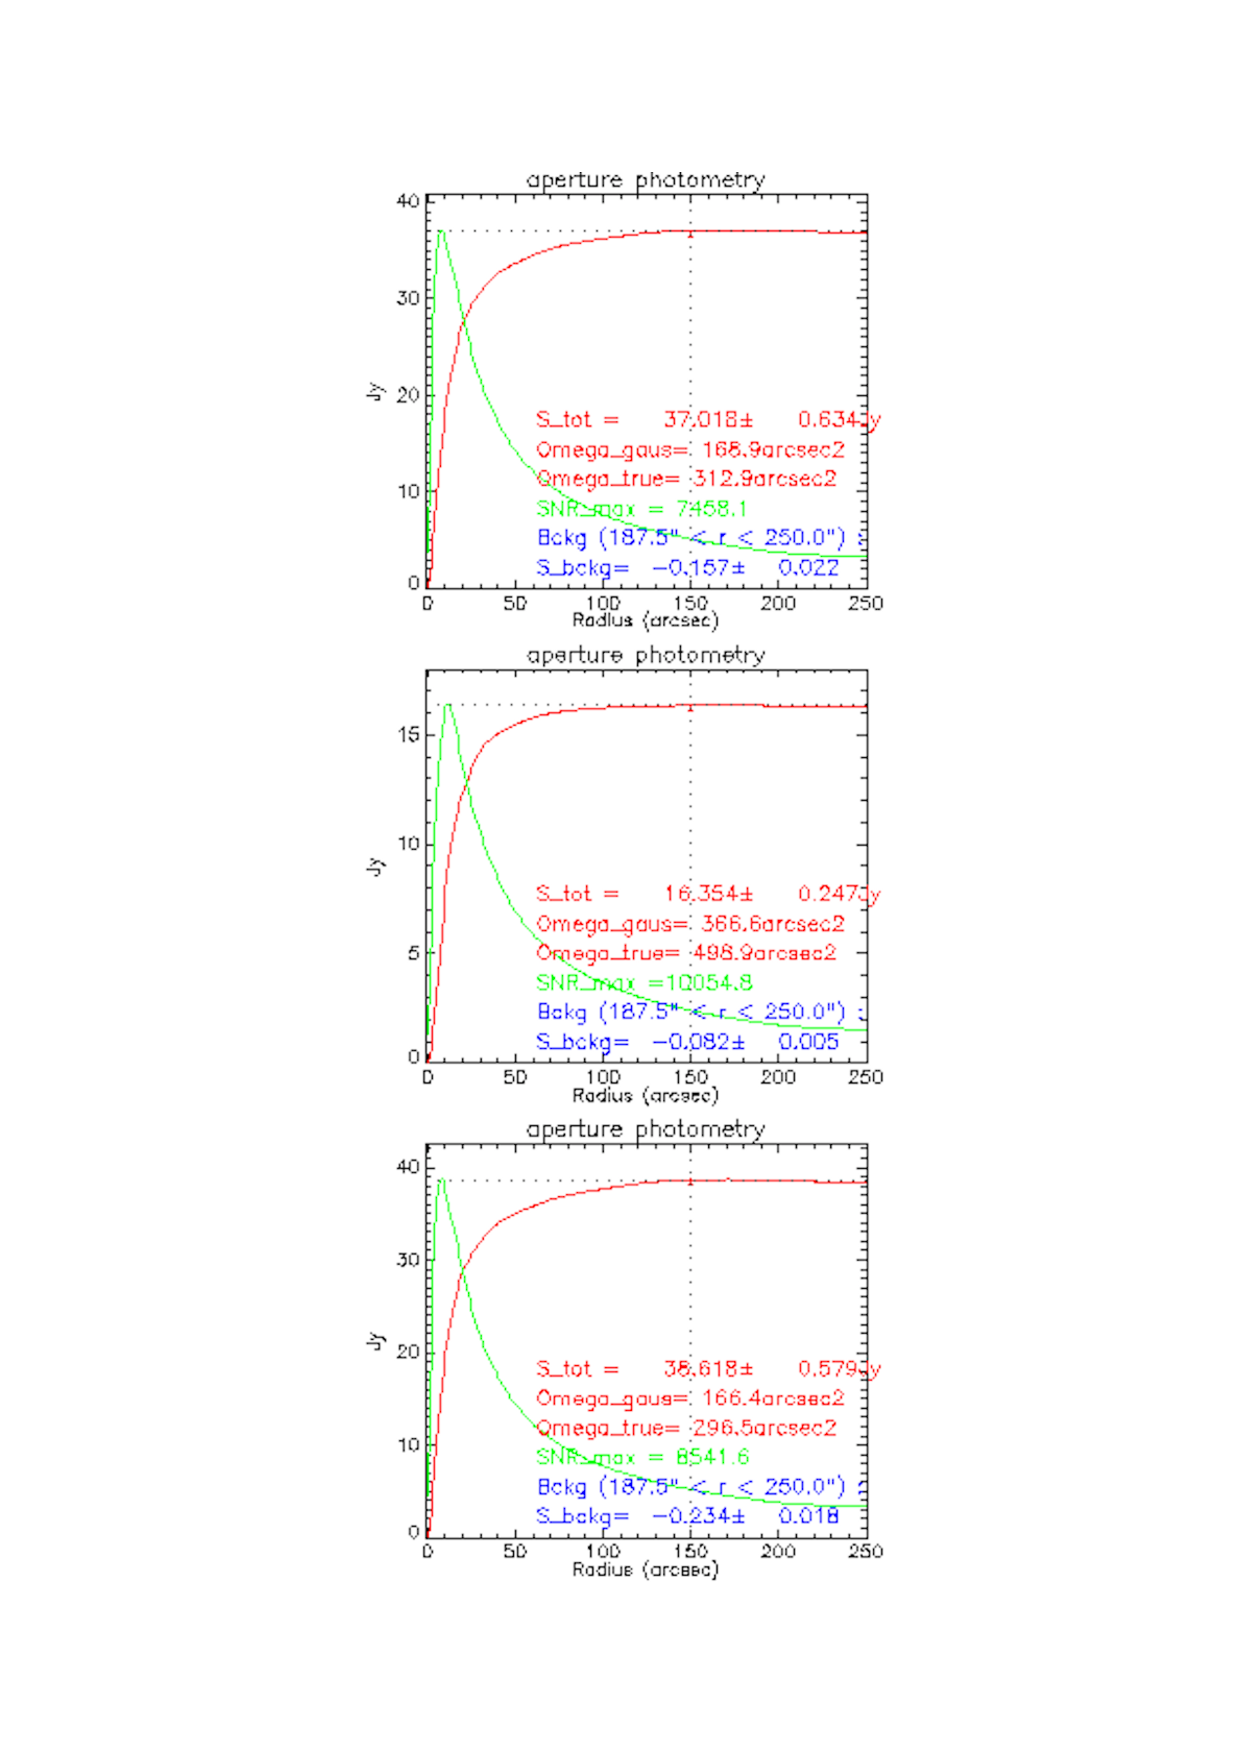
\includegraphics[clip, angle=0, scale=0.4]{Figures/Uranus_s308.pdf}
  \caption{Aperture photometry of Uranus observation 20170227s308  on array 1, 2 and 3 from top to bottom.
    The photometric curve in red saturates at about the radial distance of $150''$.
    (Green curve is the SNR in individual annulus)}
\label{fig:PhAp}
\end{center}
\end{figure}

\begin{figure}
\begin{center}
  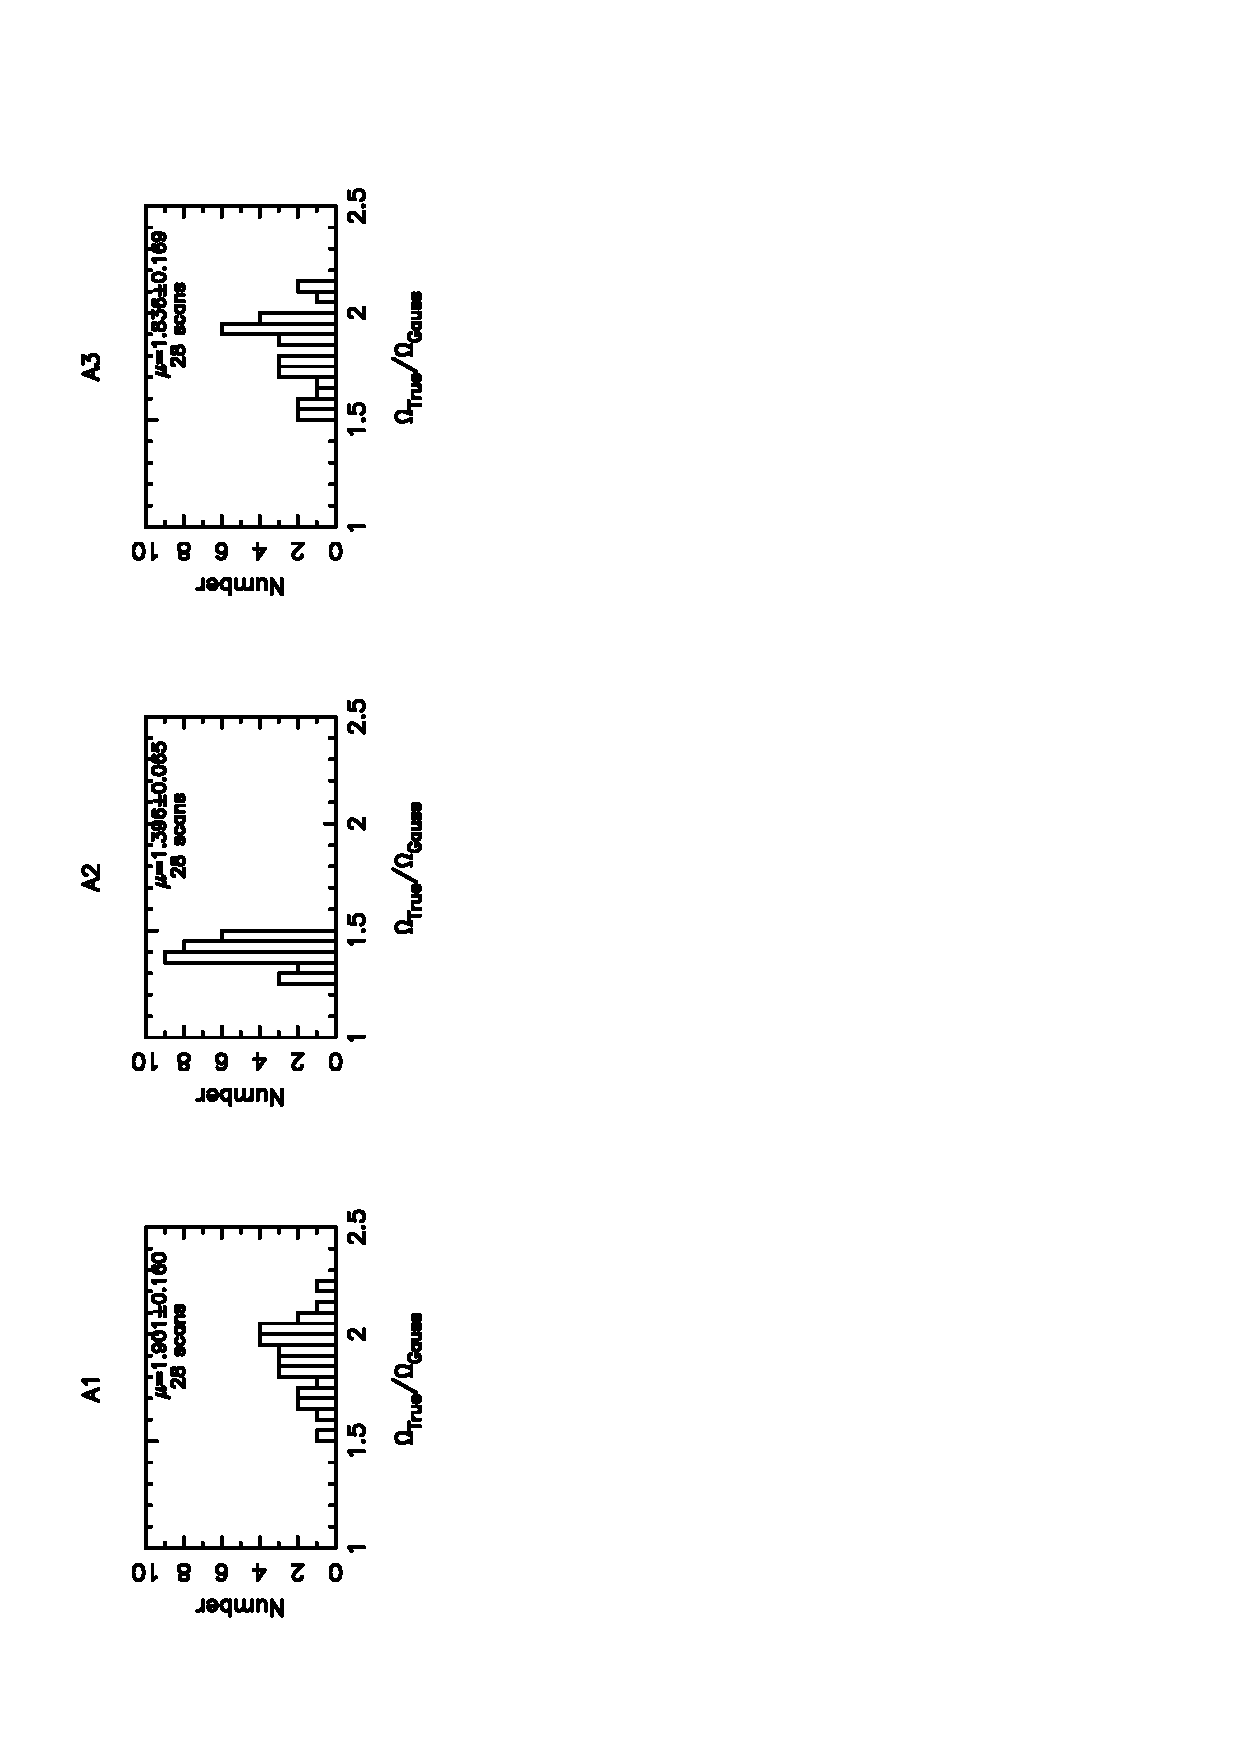
\includegraphics[clip, angle=-90, scale=0.6]{Figures/TG_hist_Ura_Nep_run9_28scan.pdf}
  \caption{Histogram of the excesses in solid angle between the true beam and the Gaussian beam for all
   observations of Uranus and Neptune during runs 9 and 10.}
\label{hist:excesses}
\end{center}
\end{figure}

\begin{figure}
\begin{center}
  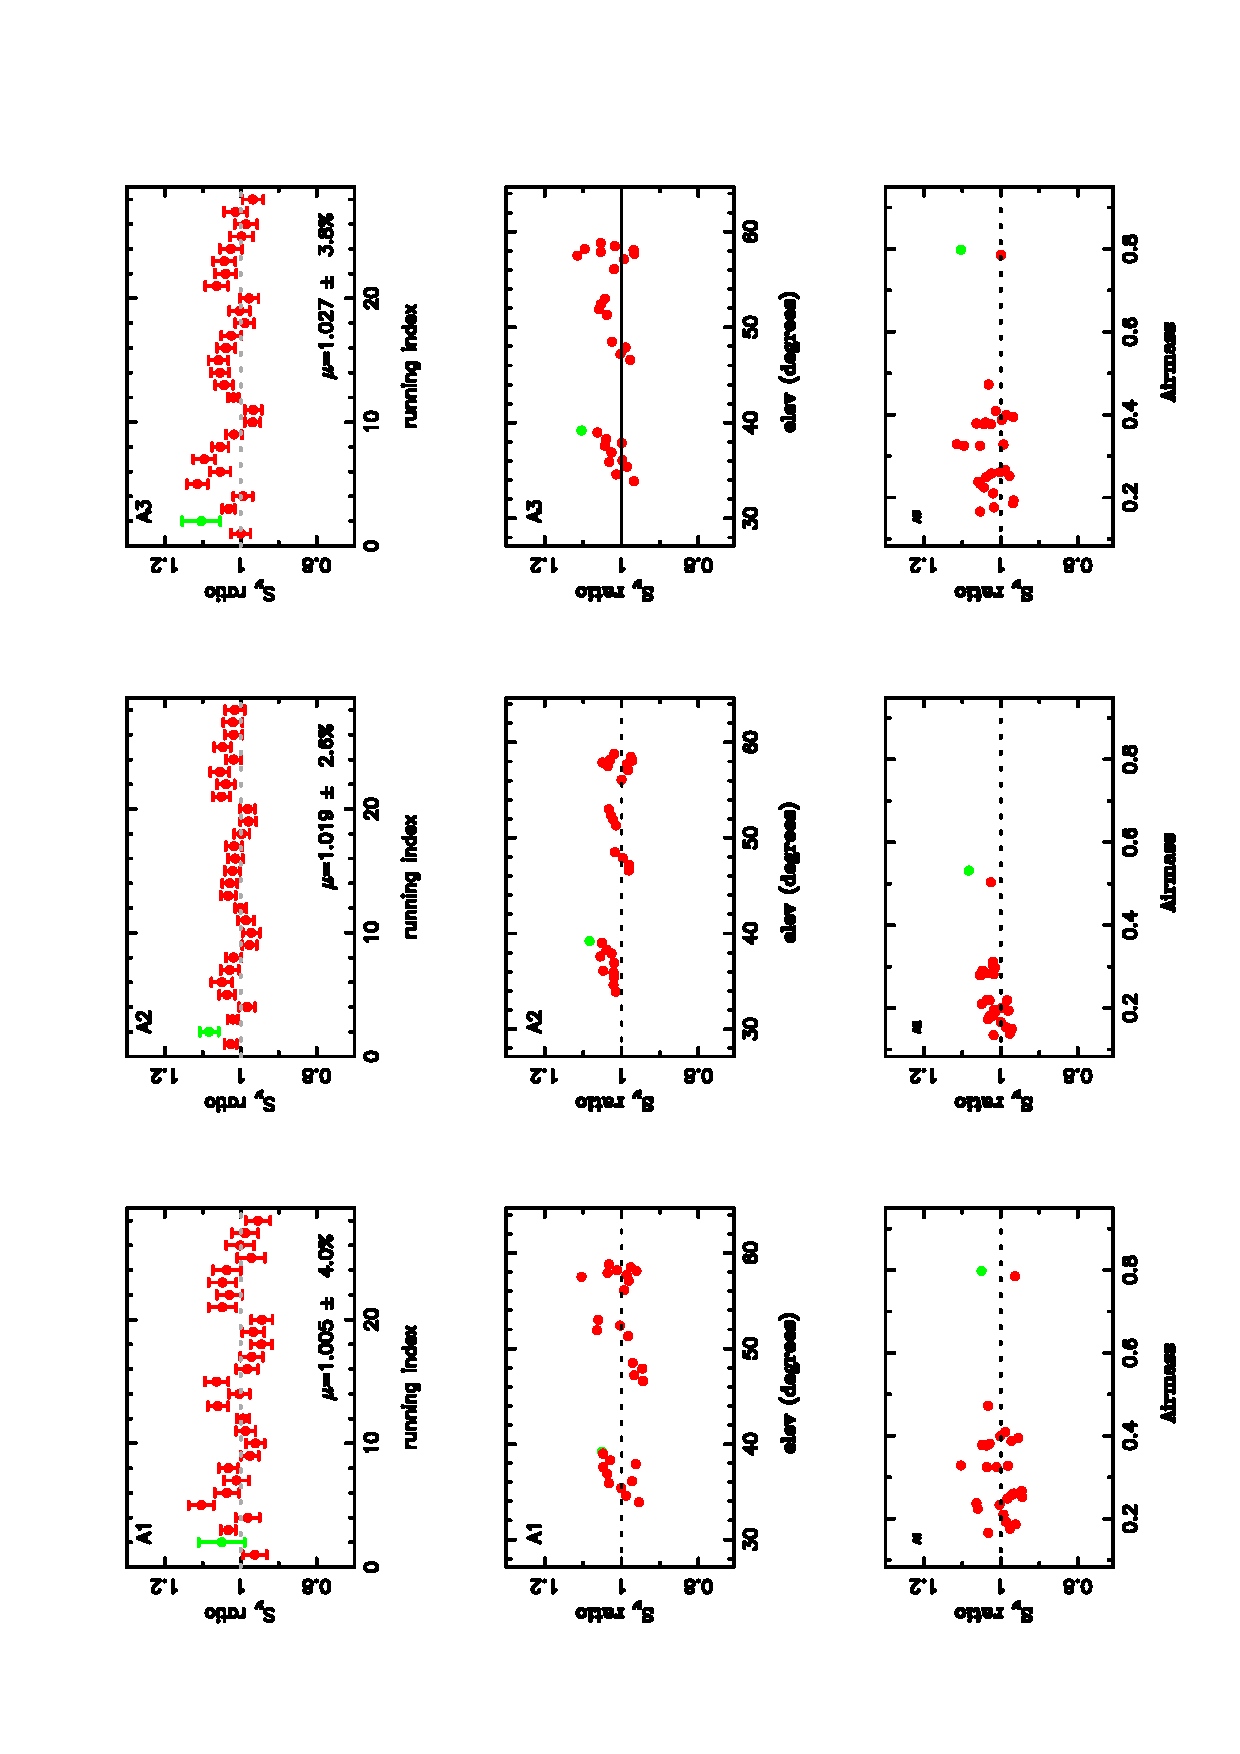
\includegraphics[clip, angle=-90, scale=0.6]{Figures/Ura_Nep_ratio_index_elev_airmass.pdf}
  \caption{Ratios between measured and reference flux densities for all observations of Uranus and Neptune during runs 9 and 10.
    Red is for Uranus and blue is for Neptune.  (DATA FILE : cal-single-obs-AZEL.dat)}
\label{fig:U_N_ratio}
\end{center}
\end{figure}

\begin{figure}
%\begin{center}                                                                                                                                               
  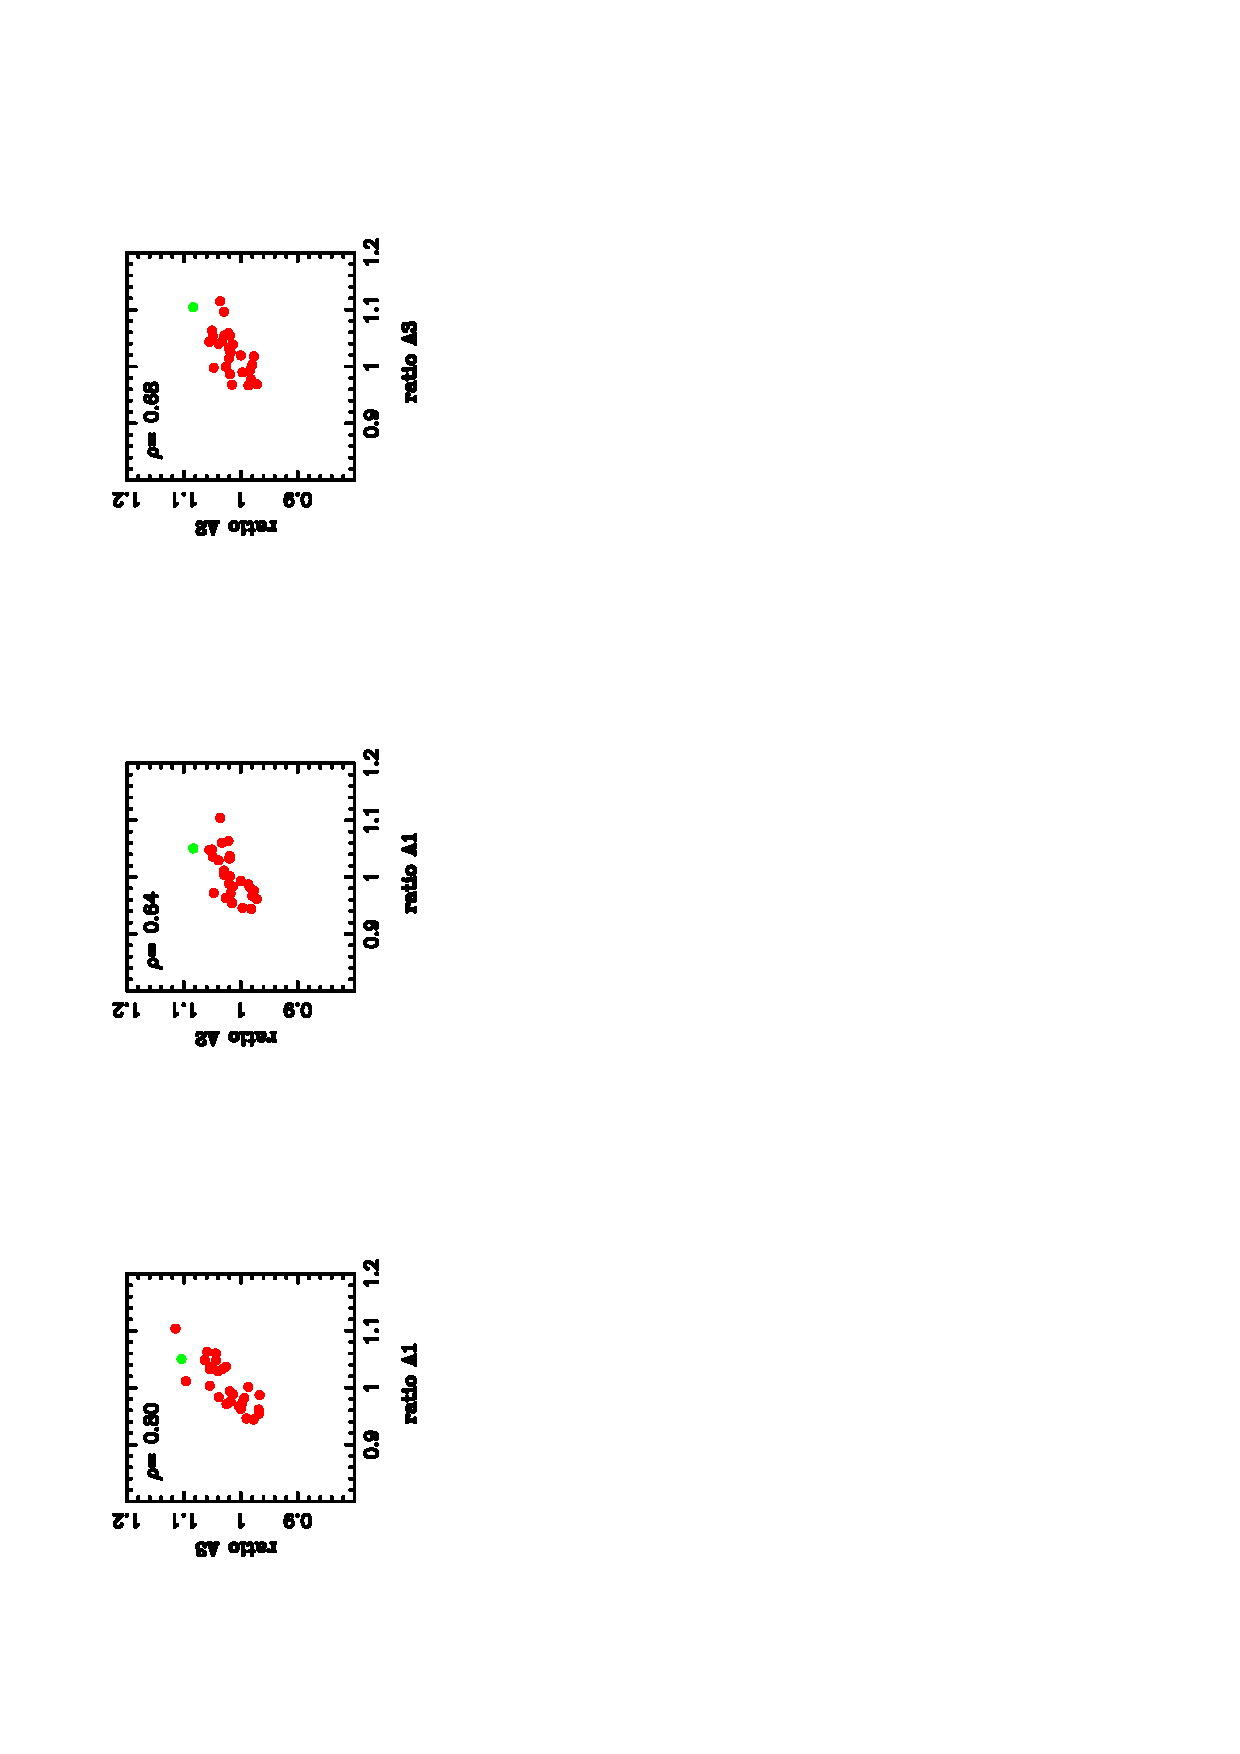
\includegraphics[clip, angle=-90, scale=0.65]{Figures/Ura_Nept_correlation_plots.pdf}
  \caption{Correlation plots between  the three arrays for all
    observations of Uranus and Neptune during run 9. Correlation
    coefficients $\rho$ are given.}
\label{fig:U_N_corr}
%\end{center}                                                                                                                                                 
\end{figure}



%We have extended this  analysis to all the secondary calibrators (Ceres, Vesta, NGC7027, MWC349, CRL2688)
%observed during run 9. As for the planets, the observations were processed with the pipeline including line-of-sight opacity.
%Aperture photometry was carried out and the solid angle $\Omega_{true}$  estimated from each map,
%except for Ceres and Vesta which are too faint. Four observations of secondary calibrators were discarded because
%aperture photometry failed to converge. The fifty three observations remaining provided flux densities on the three
%arrays that were compared to their reference flux densities given in Table~\ref{tab:fluxPred}. Their  ratios
% were plotted in Fig.~\ref{fig:all} in time order.
%The eleven flux density  measurements of CRL2688 were all clearly too high  and were multiplied
%by the factors 0.9 at 1mm and 0.75 at 2mm to yield the ratios shown in Fig.~\ref{fig:all}. Also, the flux density of Ceres at 1mm
%in Table~\ref{tab:fluxPred} is too low  but we did not correct for it because the flux densities of the four observations
%of Ceres have large uncertainties. This is apparent in the plot. The first obsertions of the strong source
%Uranus (index 1 in plot) and Neptune (index 11 in plot) in mediocre weather during the first half of the run
%do not show any degradation in the plot while secondary calibrators do. Overall,  the observations of
%all calibrators, primary and secondary, with minimal selection (four discarded out of fifty seven) and 
%a simple adjustement for calibrator CR2688, yield an absolute calibration stable  at the level
%of 14\% for array A1, 8.1\% for array A2, and 16.7\% for array A3, during run 9
%in  Fig.~\ref{fig:all}. In addition, no correlation is apparent with opacities, elevation, or airmass
%as shown in  Fig.~\ref{fig:versus_all}.






















